% --------------------------------------------------------------------------------
\newpage
\section{Roughness Module}
% --------------------------------------------------------------------------------

% Make general target
\hypertarget{Concepts:RoughnessModule}{}

% Make target for following functions:
\hypertarget{Concepts:IPEMRoughnessFFT}{}

\subsection{Introductory description}
% --------------------------------------------------------------------------------

The Roughness Module (RM) calculates the roughness (or
equivalently: the sensory dissonance) of a sound. Roughness is
considered to be a sensory process highly related to texture
perception. Hence, in our global chart of image transformation
modules it is localized in the top left (texture and sensory
based) section of figure \ref{Fig:ModulesRM}.
\begin{figure}[h]
    \centering
    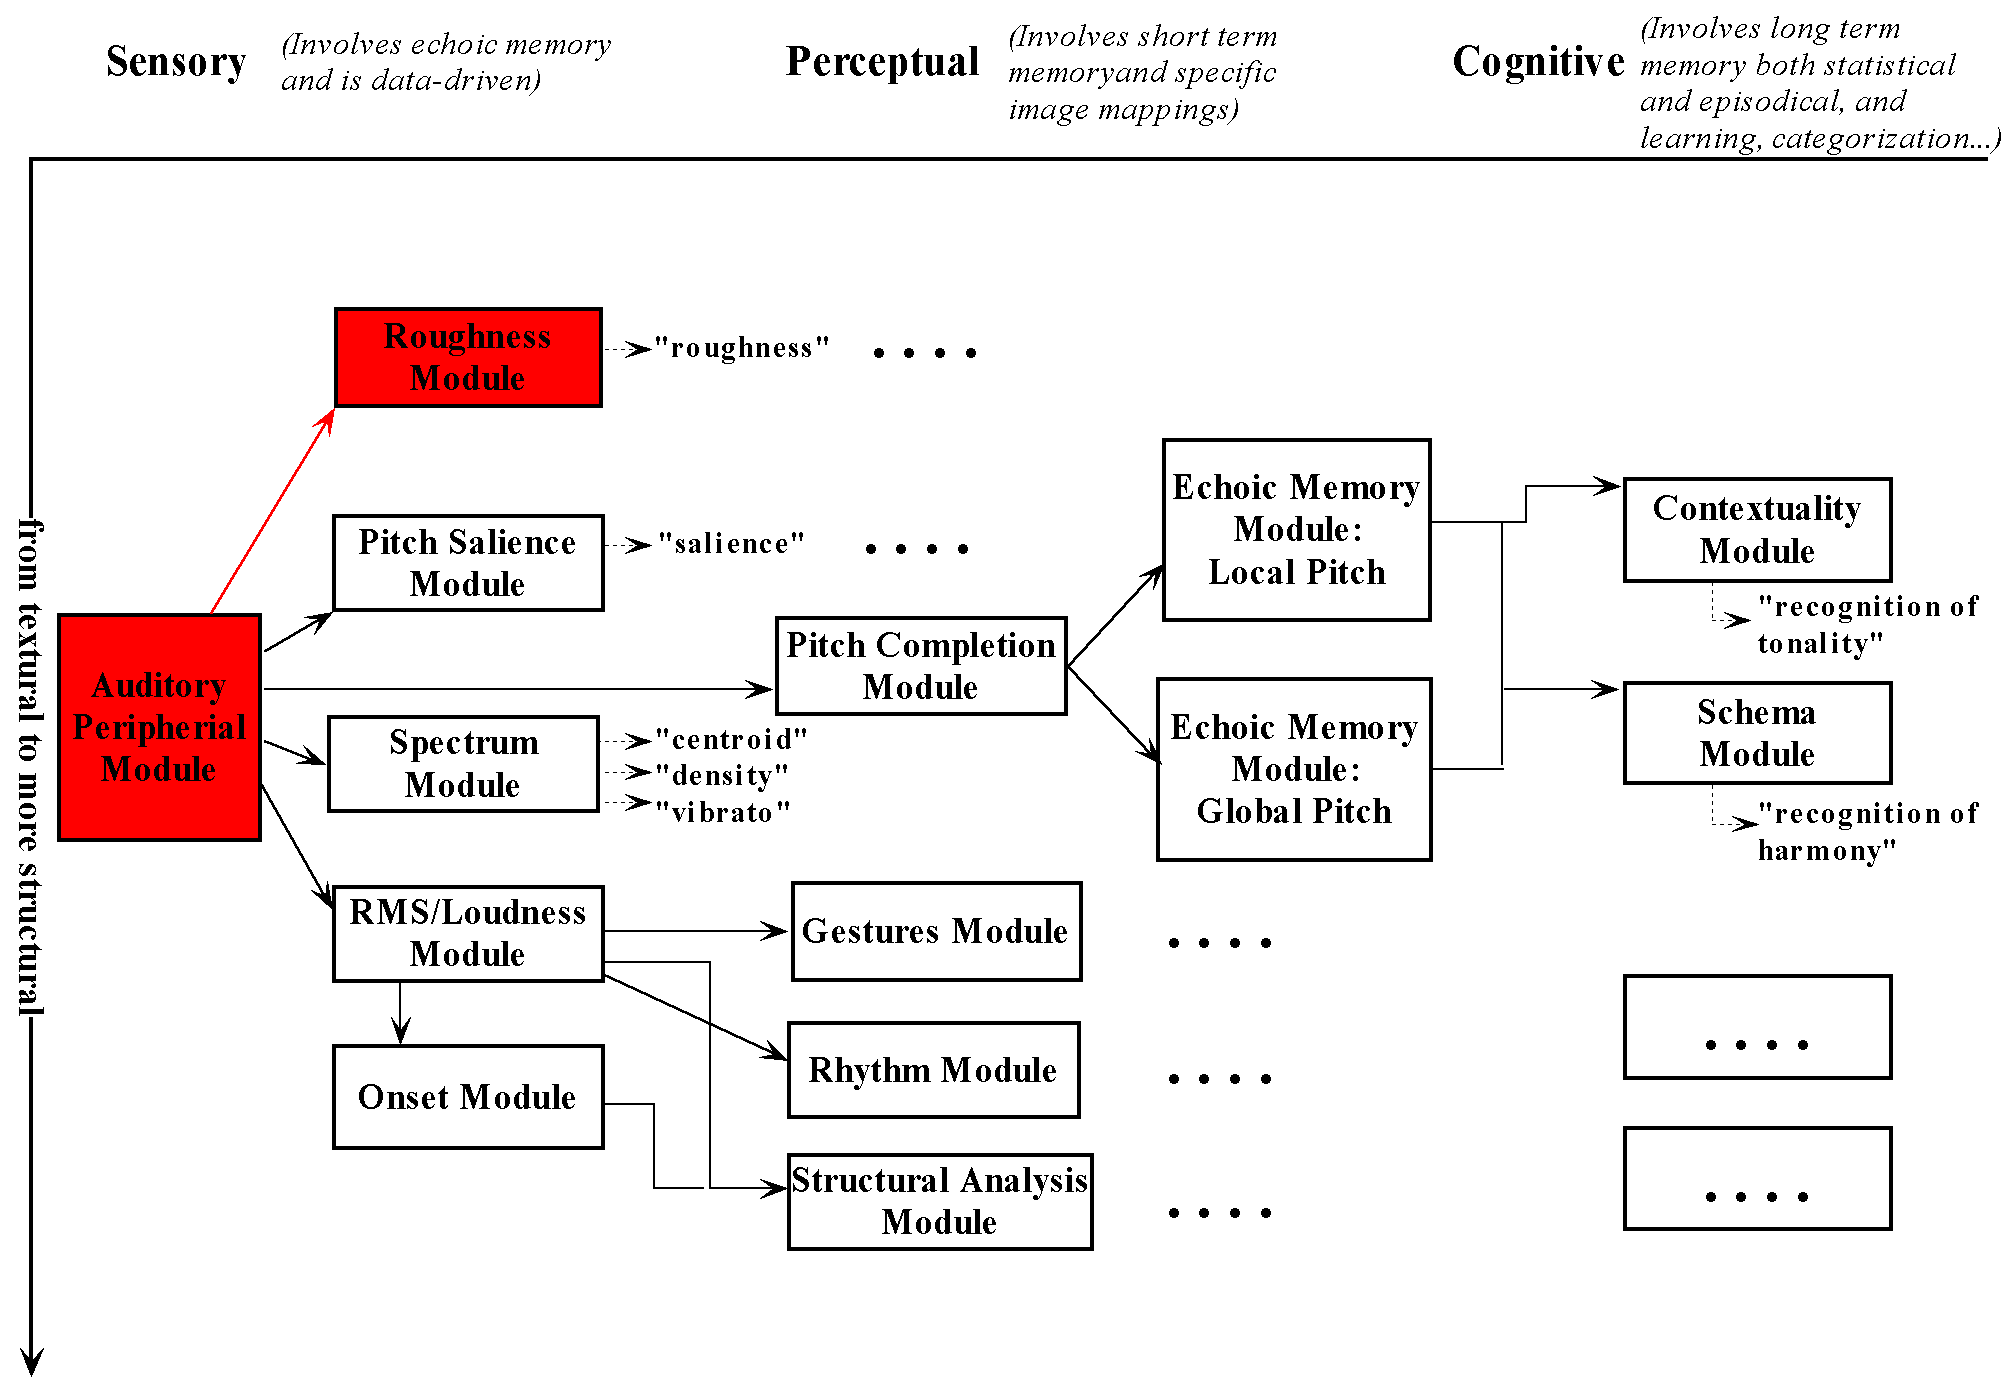
\includegraphics[width=\textwidth]{Graphics/ModulesRM}
    \caption{Chart of image transformation modules, with RM highlighted}
    \label{Fig:ModulesRM}
\end{figure}

The module takes sound as input (fig. \ref{Fig:RMModule}) and
produces a roughness estimation. The estimation should be
considered an inference.
\begin{figure}[h]
    \centering
    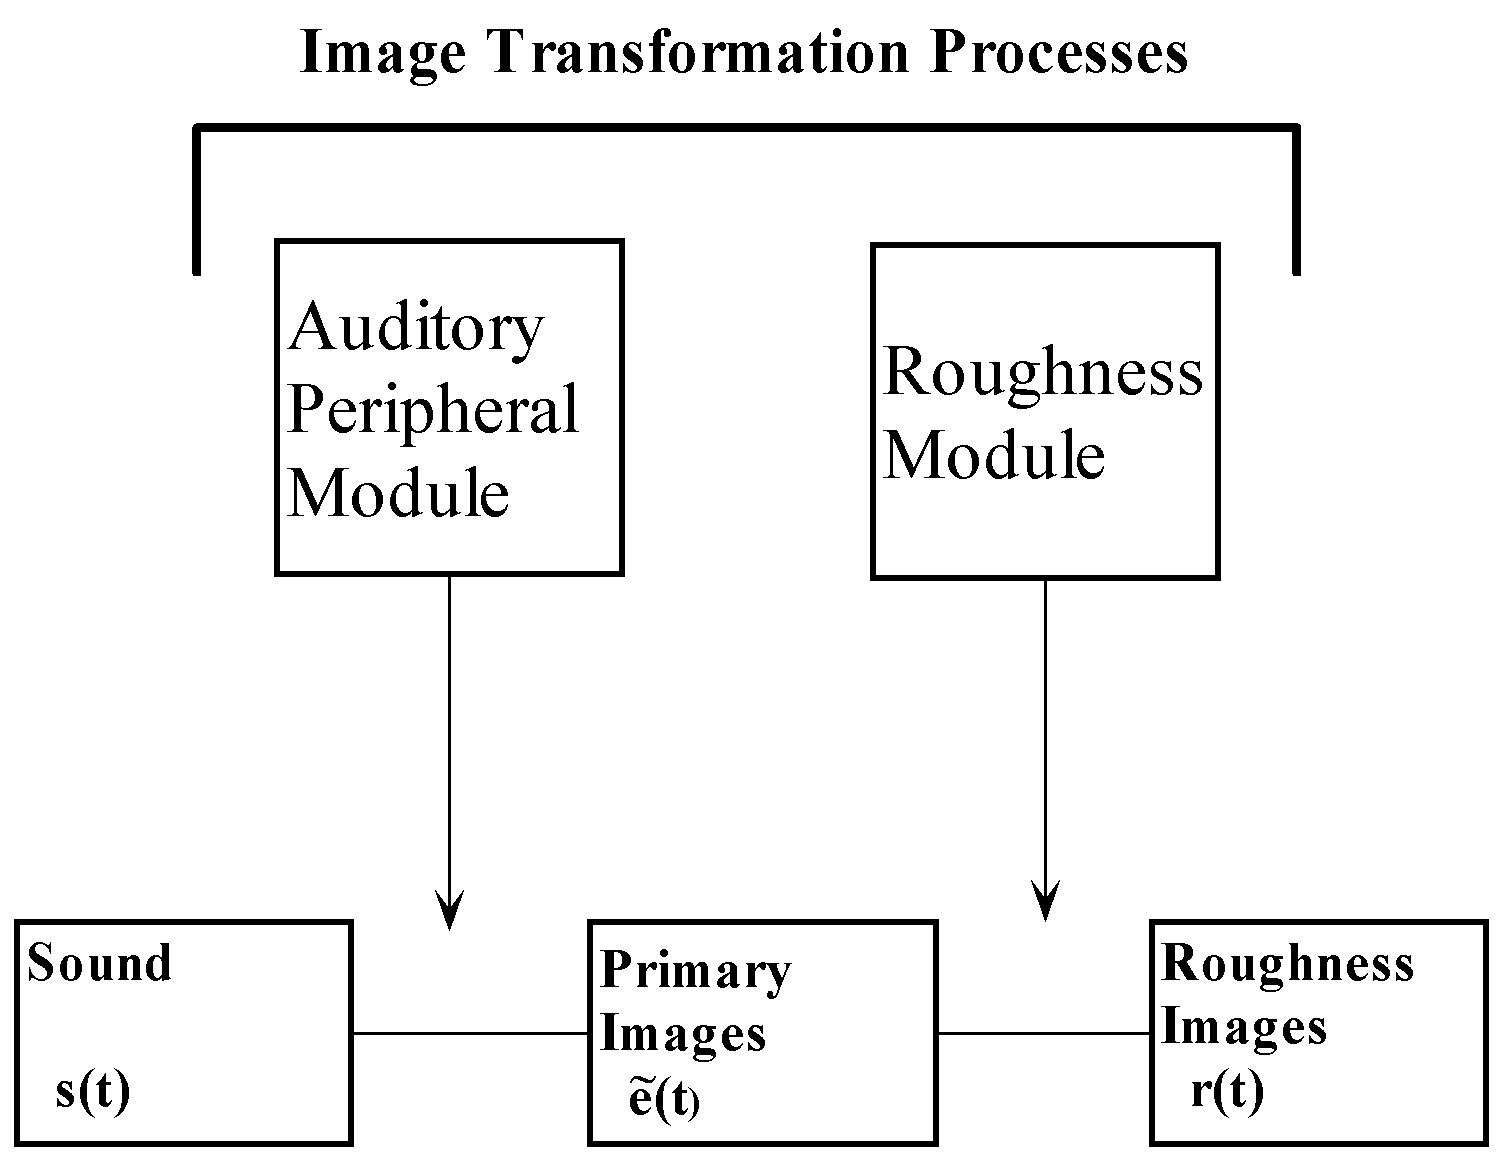
\includegraphics[width=\IPEMDefaultFigureWidth]{Graphics/RMModule}
    \caption{Image Transformation Process: Roughness Module}
    \label{Fig:RMModule}
\end{figure}
However, the module offers more than just an inference. The
visualization and calculation method of this module is based on
\citeA{inproceedings:Leman:DAFx:2000} where roughness is
defined as the energy of the relevant beating frequencies in the
auditory channels. The model is called the synchronization index
model of roughness and it is based on phase-locking to frequencies
that are present in the neural patterns. The synchronization index
model allows a straightforward visualization of the energy
components underlying roughness, in particular (i) with respect to
auditory channels, and (ii) with respect to phase-locking
synchronization (= the synchronization index for the relevant
beating frequencies on a frequency scale). That's why it is more
than just an inference. It assumes that neurons somehow extract
the energy of the beating frequencies and form internal images on
which the inference is based.

But what are beating frequencies? Take an amplitude modulated sine
wave with carrier frequency $f_c$ and modulation frequency $f_m$.
Such a signal has only three frequencies in the spectrum, in
particular $f_c$, $f_c-f_m$, and $f_c+f_m$. The beating frequency
is $f_m$. Now, in the auditory system, these frequencies are
introduced as effective beating frequencies into the spectrum of
the neural rate-code patterns. This is due to wave rectification
in the cochlea where the lower part of the modulated signal is cut
off, and as a result new frequencies are introduced of which the
most important ones correspond with the beating frequency $f_m$
and its multiples. As a matter of fact, neurons may synchronize
with these frequencies provided that they fall in the frequency
range where synchronization is physiologically possible. This
mechanism forms a physiological basis for the detection of beats
and hence, the sensation of roughness.

According to \citeA[p.~520-521]{Javel:88}, the synchronization
index represents the degree of phase-locking to a particular
frequency that is present in the neural pattern. The index can be
mathematically expressed as the (normalized) Fourier Series
coefficient at the frequency of interest. Using this concept, the
degree of roughness can be defined as the sum of the normalized
magnitudes or 'energies' of the relevant beating frequencies in
the Fourier spectrum.


\subsection{Functional-logical description}
% --------------------------------------------------------------------------------

Strictly speaking the roughness module realizes a transformation
from auditory nerve images onto roughness values. In a broad sense
the module starts from sound involving:
\begin{eqnarray}
    APM: s(t) \rightarrow \tilde{e}(t)\\
    RM: \tilde{e}(t) \rightarrow r(t)
\end{eqnarray}
where APM is the Auditory Peripheral Module which is used as the
first step, and RM is the transformation from the primary images
$\tilde{e}(t)$ to the roughness values $r(t)$ (our Roughness
Module in the strict sense). The latter are scalar values which we
can compare with human behavioral outputs.

\subsection{Signal processing description}
% --------------------------------------------------------------------------------

The synchronization index model calculates roughness in terms of
the 'energy' of neural synchronization to the beating
frequencies. The 'energy' refers to a quantity which we derive
from the magnitude spectrum.

Since the beating frequencies are contained in the lower
spectral area of the neuronal pattern $e(t,c)$, the spectral
part we are interested in is defined as:
\begin{equation}
  B(t,f,c) ~=~ F(f,c)D(t,f,c)
\end{equation}
where $F(f,c)$ is a filter whose spectrum is depending on the
channel $c$, and $D(t,f,c)$ is the short-term spectrum in
channel $c$ which we define as:
\begin{equation}\label{E1}
  D(t,f,c)~=~\int_{-\infty}^{+\infty} e(t,c)w(t'-t)e^{-j2\pi
  ft'}~dt'
\end{equation}
where $e(t,c)$ is the neural pattern in channel $c$, and
$w(t'-t)$ is a (hamming) window. The \emph{magnitude} spectrum
is then defined as $\left|~D(t,f,c)~\right|$, and the
\emph{phase} spectrum as $\angle D(t,f,c)$.

In order to be able to reproduce the psychoacoustical data on
roughness, the filters $F(f,c)$ should be more narrow at auditory
channels where the center frequency is below 800 Hz, and the
filters should be attenuated for high center frequencies as
well. The proposed set of filters $F(f,c)$ are shown in figure
\ref{Fig:Filters}. Small changes in parameters do not have a
dramatic effect on the performance of the model.

\begin{figure}[ht]
    \centering
    \includegraphics[width=\IPEMDefaultFigureWidth]{Graphics/Filters}
    \caption{Filters become more narrow in the lower auditory channels.}
    \label{Fig:Filters}
\end{figure}



$B(t,f,c)$ represents the \emph{spectrum} of the neural
synchronization to the beating frequencies in channel $c$. The
\emph{synchronization index} of the beating frequencies is then
defined as the normalized magnitude:
\begin{equation}
  I(t,f,c) ~=~ \left |~ \frac{B(t,f,c)}{D(t,0,c)}~\right |
\end{equation}
where $I(t,f,c)$ is the normalized magnitude in channel $c$.
$D(t,0,c)$ is the DC-component of the whole signal in channel
$c$.

The short-term \emph{'energy'} spectrum of the neural
synchronization to beating frequencies in a particular auditory
channel $c$ is defined as:
\begin{equation}\label{Rspectrum}
\textbf{B}(t,f,c) ~=~ I(t,f,c) ~^{1.6}~=~ {\left |~
\frac{B(t,f,c)}{D(t,0,c)}~\right |~}^{1.6}
\end{equation}

%\item
% the energy spectrum of the neural synchronization to
% beating frequencies over all auditory
% channels is:
%\begin{equation}\label{R2}
%\textbf{B}(t,f) ~=~ \sum_{c=1}^{C} \textbf{B}(t,f,c)~ w_c
%\end{equation}
%where $w_c$ is the weighting factor defined for each channel.
%\item
% the overall energy of the neural synchronization to beating frequencies in one channel is:
% \begin{equation}\label{R3}
%E_\textbf{B}(t,c) ~=~ \int_{f=-\infty}^{+\infty}
%\textbf{B}(t,f,c)~df
%\end{equation}
%\end{itemize}



We then define the following relationships for the calculation of
roughness:
\begin{equation}\label{R5}
\begin{array}{lll}
  R_\textbf{B}(t)&~=~\int \textbf{B}(t,f)~df
                 &~=~\int \sum_{c=1}^{C}
                 \textbf{B}(t,f,c)~df\\\\
                 &~=~\sum_{c=1}^{C} \textbf{B}(t,c)
                 &~=~\sum_{c=1}^{C} \int  \textbf{B}(t,f,c)~df\\
\end{array}
\end{equation}
where $R_\textbf{B}(t)$ is the roughness at time $t$. The
roughness is obtained by an integration of the 'energy' over all
frequencies, as well as over all channels. This definition
implies a proper visualization, one along the axis of auditory
channels and one along the axis of the (beating) frequencies.

%We now assume that roughness is related to the 'energy' of this
%normalized Fourier transform.
%
%In particular, roughness is calculated in the individual channels
%and the total roughness is the sum of the channel roughnesses.
%Given the above discussion, it will be possible to visualize the
%contribution of the synchronization energy along the axis of the
%auditory channels, as well as along the axis of the beating
%frequencies.






%Given the general concept as described above, the implementation
%requires a specification of the filters $F(f,c)$. In the present
%modeling, we choose elegance as an important criterium to
%describe the filters mathematically.
%The form of the filter
%$F'(f,c)$ has first been defined according to the following
%formula's:
%\begin{equation}
%F'(f,c)~=~e^{-8 \frac{f}{f_B}} \left [~1 - cos(2 \pi
%\frac{f}{10f_B}) ~\right ] w(c)
%\end{equation}
%where $f_B$ is the frequency range of the filter and $f$ is
%running from 1 to $f_B$, $w(c)$ is a weight depending on the
%channel $c$. The weight takes into account a linear decrease of
%the impact of the filter depending on the auditory channel number:
%\begin{equation}
%w(c)~=~1-\frac{0.55c}{C})
%\end{equation}
%with c running from 1 to C (=40). The frequency range $f_B$ is
%defined such that it is narrow for the lower auditory channels
%below 800 Hz, broad at about 1000 Hz and again slightly more
%narrow at frequencies higher than 1500 Hz.
%
%A sigmoid function has been defined according to
%%(fig.~\ref{Sigmoid}):
%\begin{equation}\label{Sigmoid}
%S~=~ \frac{(\frac{c}{C})^{.2}} {0.04 + (\frac{c}{C})^{2.45} -
%0.007c}
%\end{equation}
%The sigmoid function is used to define the frequency range as:
%\begin{equation}
%f_B(c) = 10 + (300 * \frac{S}{S_{max}} );
%\end{equation}
%It means that the frequency range of the filter in the lowest
%auditory channel is 10 Hz, and that this range is at most 310 Hz
%(around 1000 Hz). The values of S are normalized so that the
%maximum value of $\frac{S}{S_{max}}$ is equal to one.
%
%%\begin{figure}
%%  \centering
%%  \includegraphics{figures/Sigmoid}
%%  \caption{Sigmoid function}\label{Sigmoid}
%%\end{figure}
%Given the set of filters $F(f,c)$, the sigmoid function
%(\ref{Sigmoid}) has also been used to define where the maximum of
%the filter should be located. Data indicate that the maximum
%around 1000 Hz is at about 70 Hz. It is lower for low auditory
%channels.
%\begin{equation}
%f_M(c) = 20 + (52 * \frac{S}{S_{max}} );
%\end{equation}
%This function starts at 20 Hz and the maximum is obtained at 72
%Hz.
%
%The precise location of the filter shape $F'(f,c)$ on the
%frequency axis is then determined by placing its maximum at
%$f_M(c)$.



%Figure \ref{Filters} shows an array of such filters.
%\begin{figure}
%  \centering
%  \includegraphics{figures/Filters}
%  \caption{Filters become more narrow in the lower auditory channels}\label{Filters}
%\end{figure}


\subsection{Implementation}
% --------------------------------------------------------------------------------

\begin{tabularx}{\linewidth}{llX}
\hyperlink{FuncRef:IPEMRoughnessFFT}{IPEMRoughnessFFT} & - & Calculates roughness using synchronization index model\\
\end{tabularx}


\subsection{Examples}
% --------------------------------------------------------------------------------

The function
\hyperlink{FuncRef:IPEMRoughnessFFT}{IPEMRoughnessFFT}
has a number of input parameters. To calculate the roughness of
the wav-file \emph{SchumannKurioseGeschichte.wav} do:\\

\IPEMCodeExtract{[ANI,ANIFreq,ANIFilterFreqs] = ...\\IPEMCalcANIFromFile('SchumannKurioseGeschichte.wav');}\\

\IPEMCodeExtract{IPEMRoughnessFFT(ANI,ANIFreq,ANIFilterFreqs,5,300,0.200,0.020,1);}\\

Notice that the toolbox functions are linked through the variables
\IPEMCodeExtract{ANI,ANIFreq,ANIFilterFreqs}. These variables are
the output of the Auditory Peripheral Module, and (part of) the
input to the Roughness Module. The resulting figure should be
similar to the one shown in figure \ref{Fig:RMRoughness}.\\

\begin{figure}[h]
    \centering
    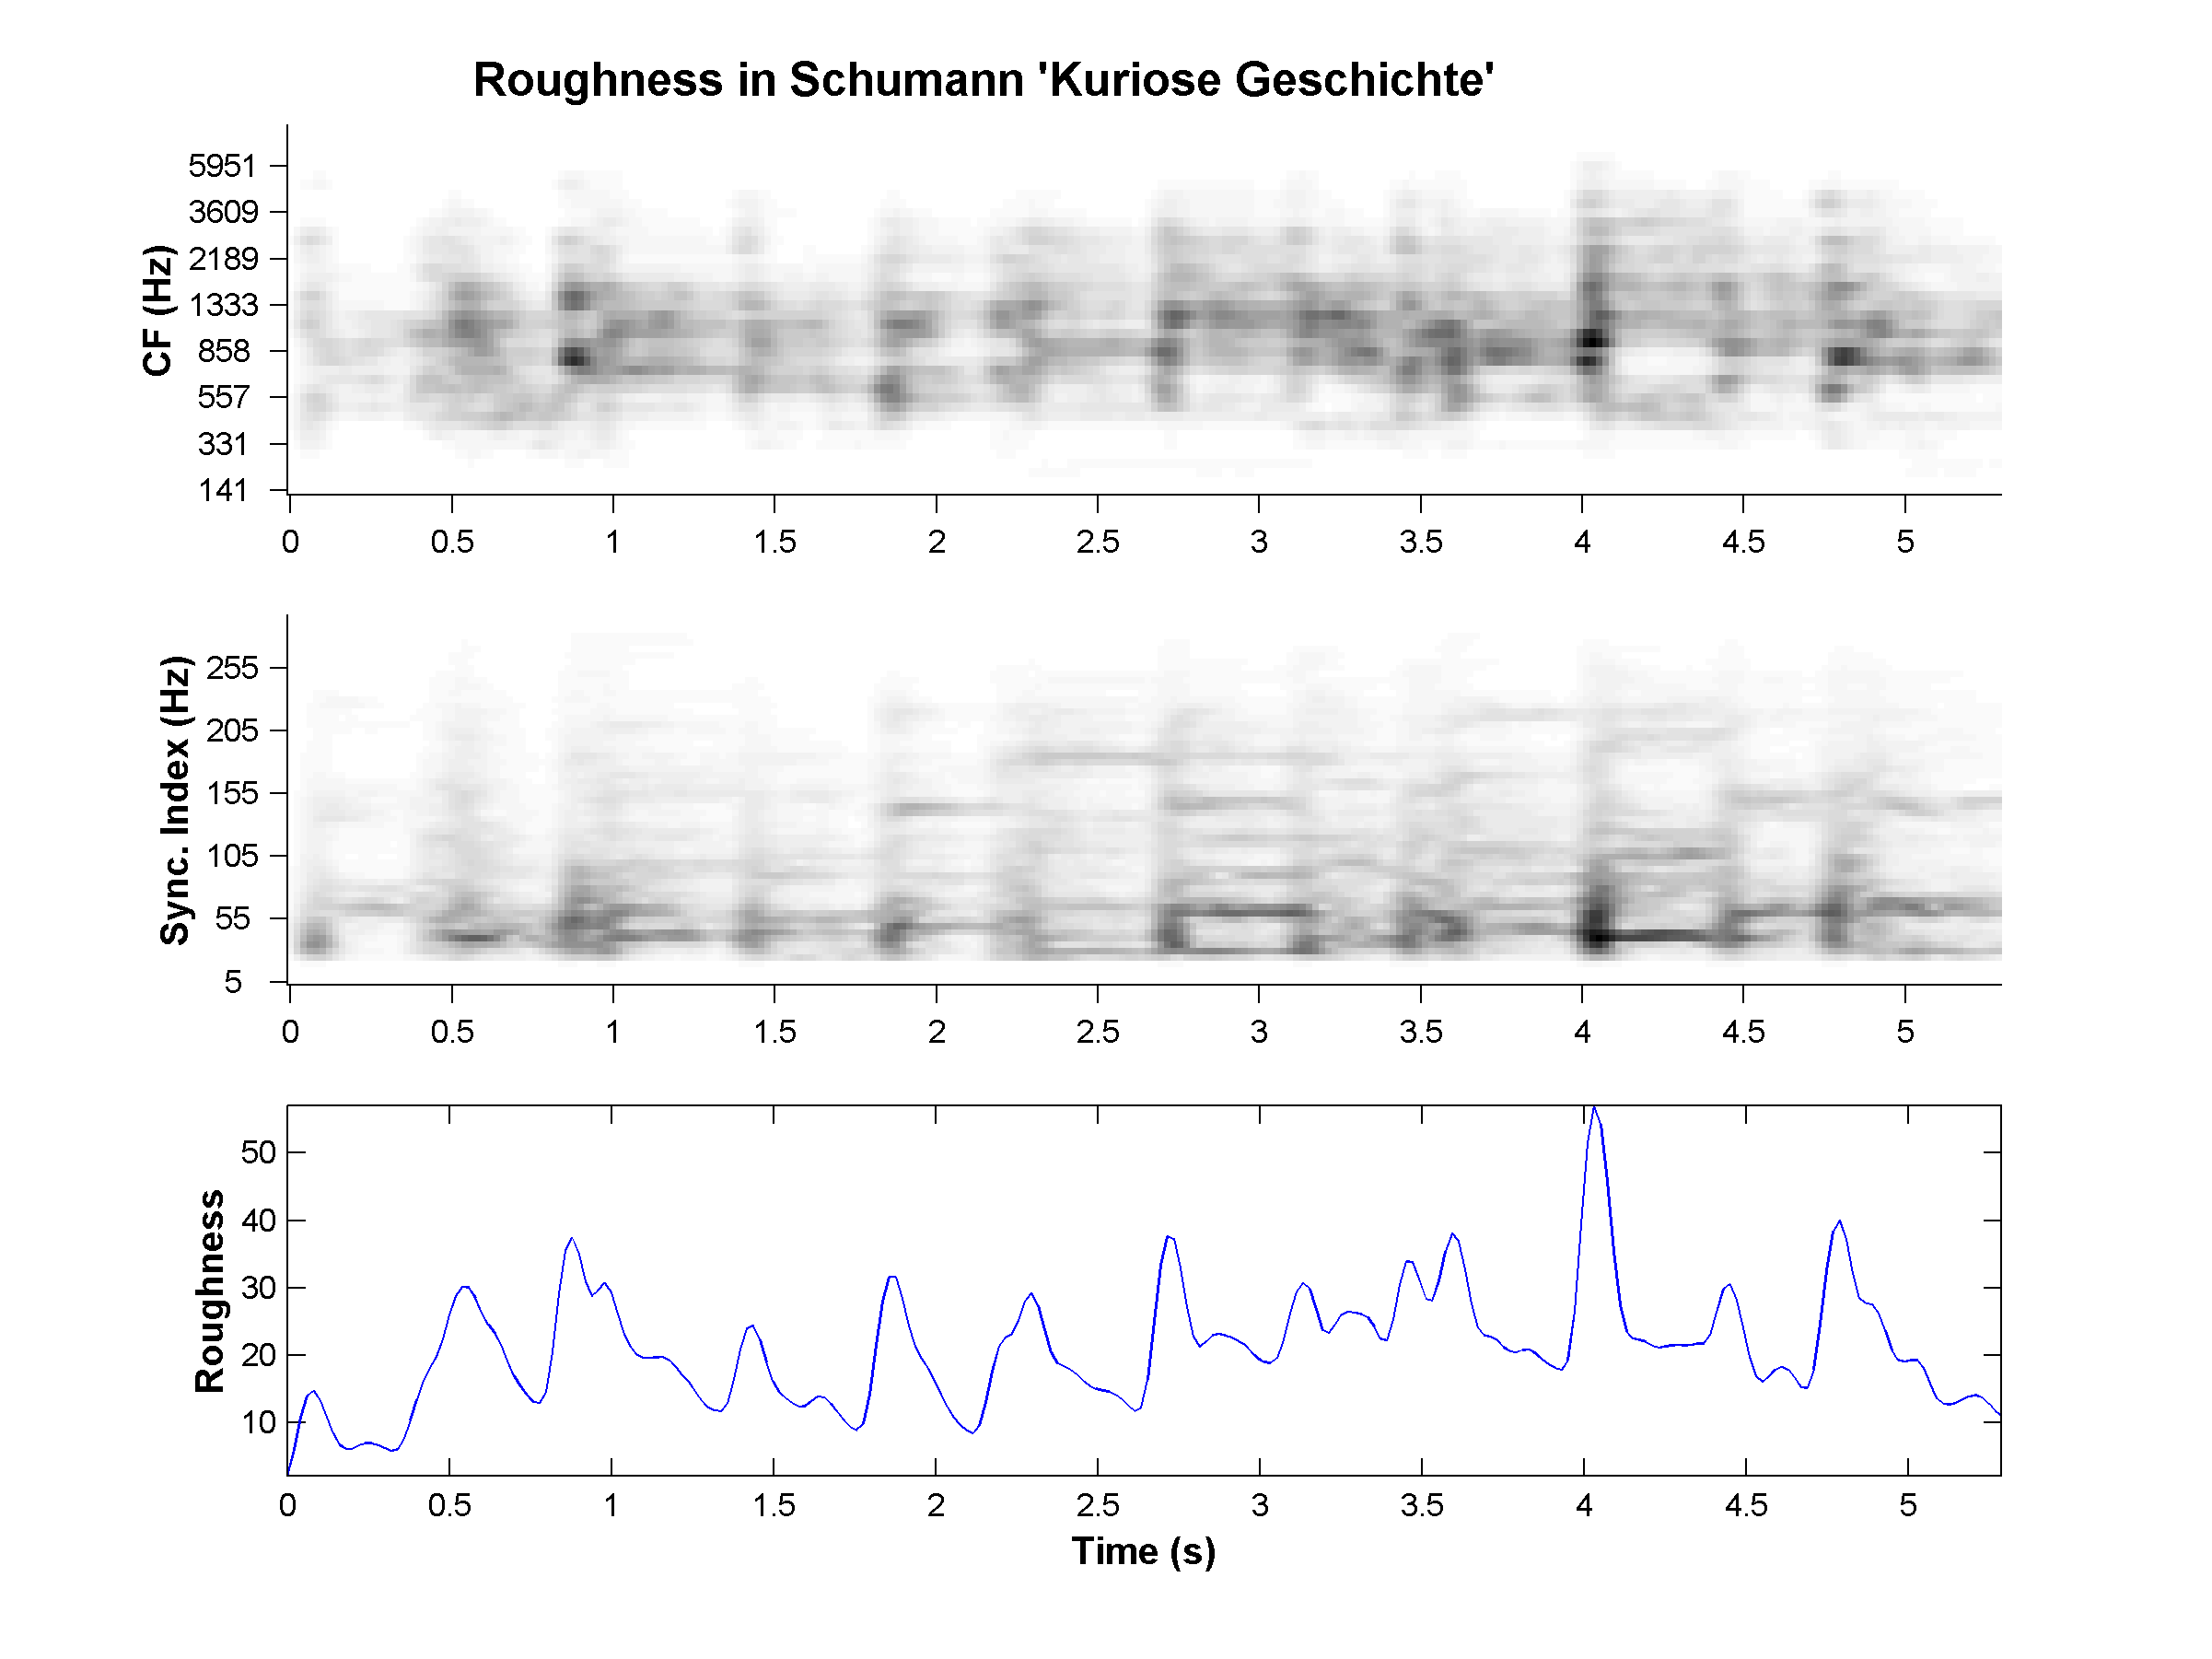
\includegraphics[width=\IPEMDefaultFigureWidth]{Graphics/RMRoughness}
    \caption{The upper panel shows the energy as distributed over the
    auditory channels, the middle panel shows the energy as
    distributed over the beating frequencies, the lower panel
    shows the roughness (which is the sum of either the upper or
    middle panel)}
    \label{Fig:RMRoughness}
\end{figure}

%See also \hyperlink{Chapter:ConceptsApplications}{Applications}
%for more elaborate examples.\\
